\section{A brief overview of the analysis}
\label{sec:overview}

As previously mentioned, the polarization measurement is made by fitting Eq.~\ref{eq:W}
to the measured \abscosth distribution, after correcting it for acceptance and efficiency effects, 
which is done by dividing it by the corresponding MC distribution.
Given that the analysis is made as a function of \pt, we can say that the basic inputs for the
polarization measurement are the two-dimensional \abscosth vs.\ \pt event distributions,
for the data and for the MC.

Figure~\ref{fig:2Dmaps_data_vs_MC}-left shows the \jpsi \abscosth vs.\ \pt event distribution 
measured with the 2018 event sample, for the Peak region,
after applying all the event selection criteria. 
In this kind of "2D map" representation, 
the analogous distributions for the NP region and for the 2017 data taking period
are virtually indistinguishable from the one shown here.
%
The corresponding MC distribution, for the 2018 conditions,
is shown in Fig.~\ref{fig:2Dmaps_data_vs_MC}-right. 
Since the MC samples are generated unpolarized, 
the non-flatness of this distribution versus \abscosth is a direct reflection of the detection acceptance.
The measured data, instead, is also affected by the physics polarization effects
that we are interested in measuring.

\begin{figure}[h]
\centering
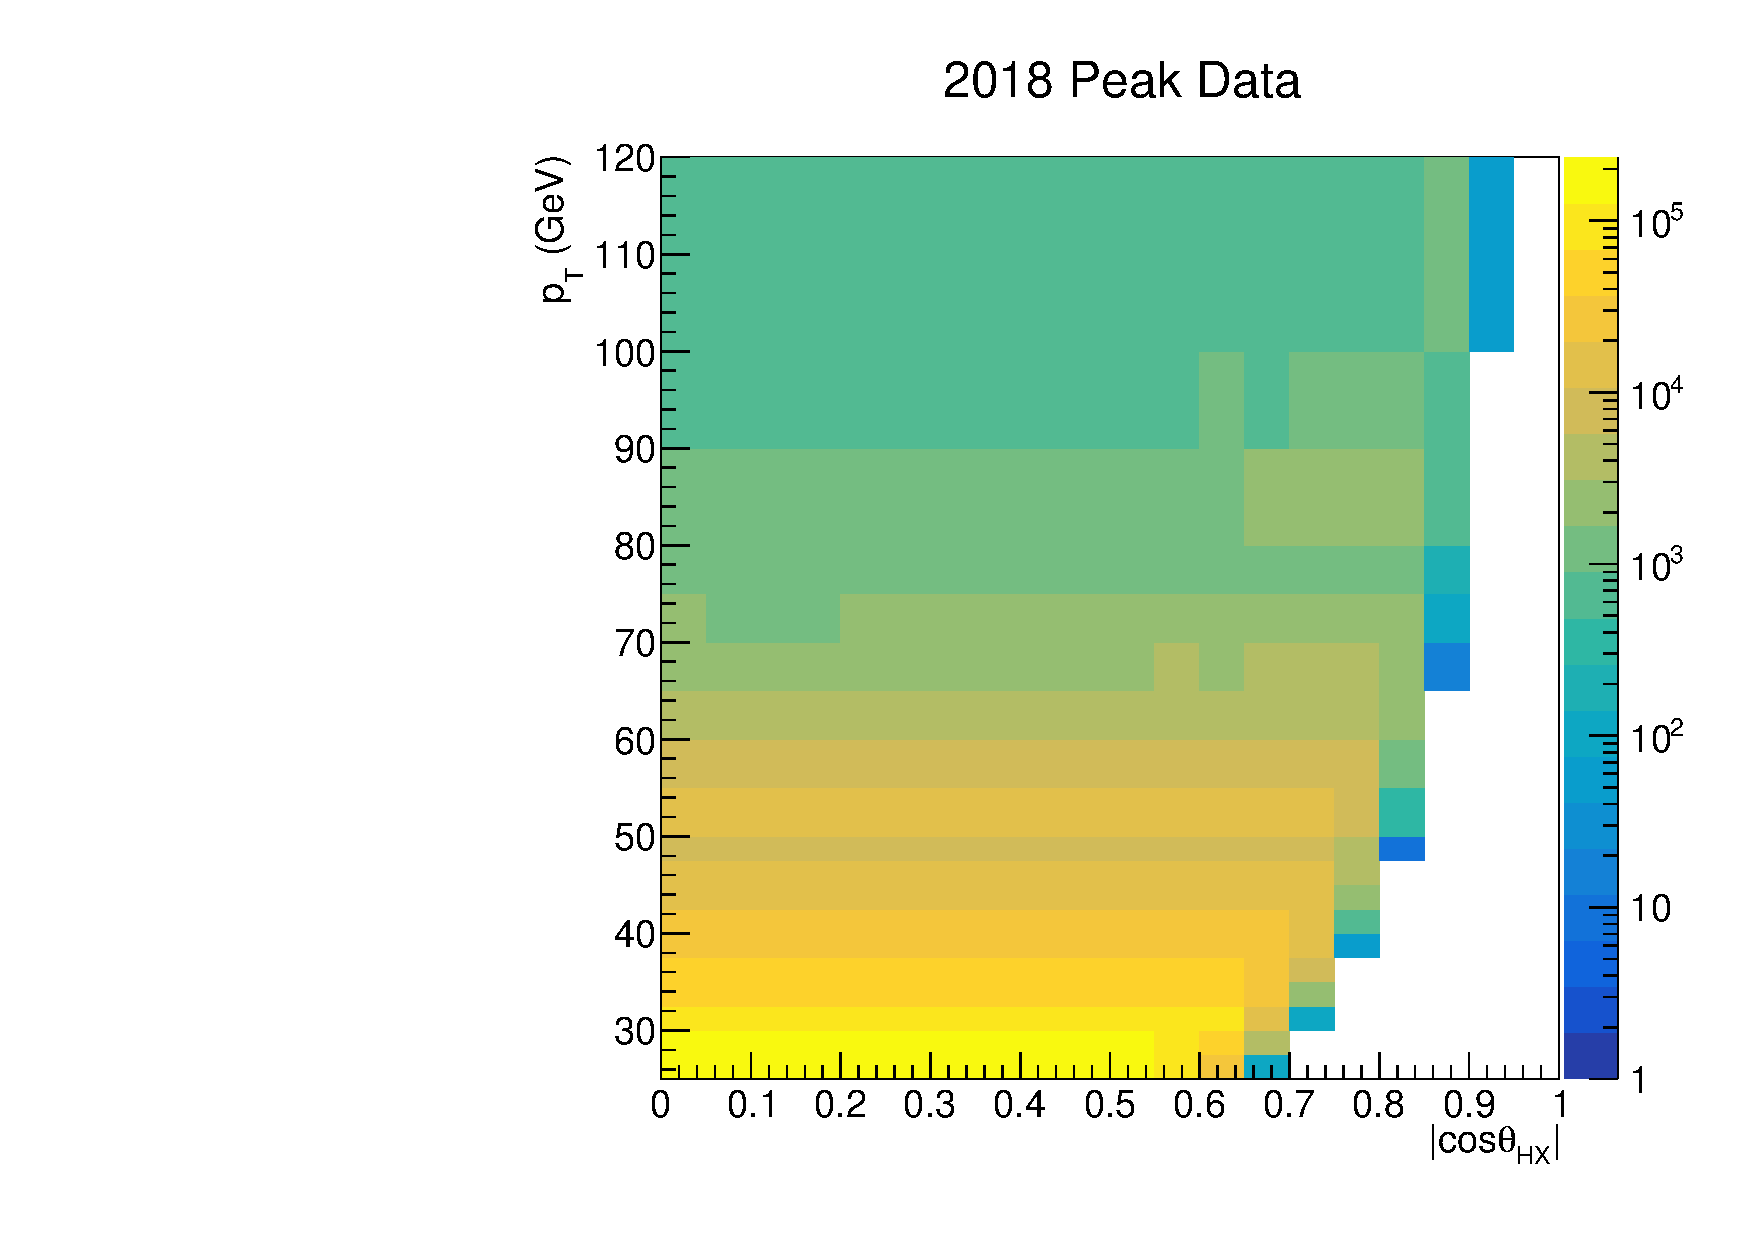
\includegraphics[width=0.48\textwidth]{Figures/chapter3/data_2d_plot.pdf}
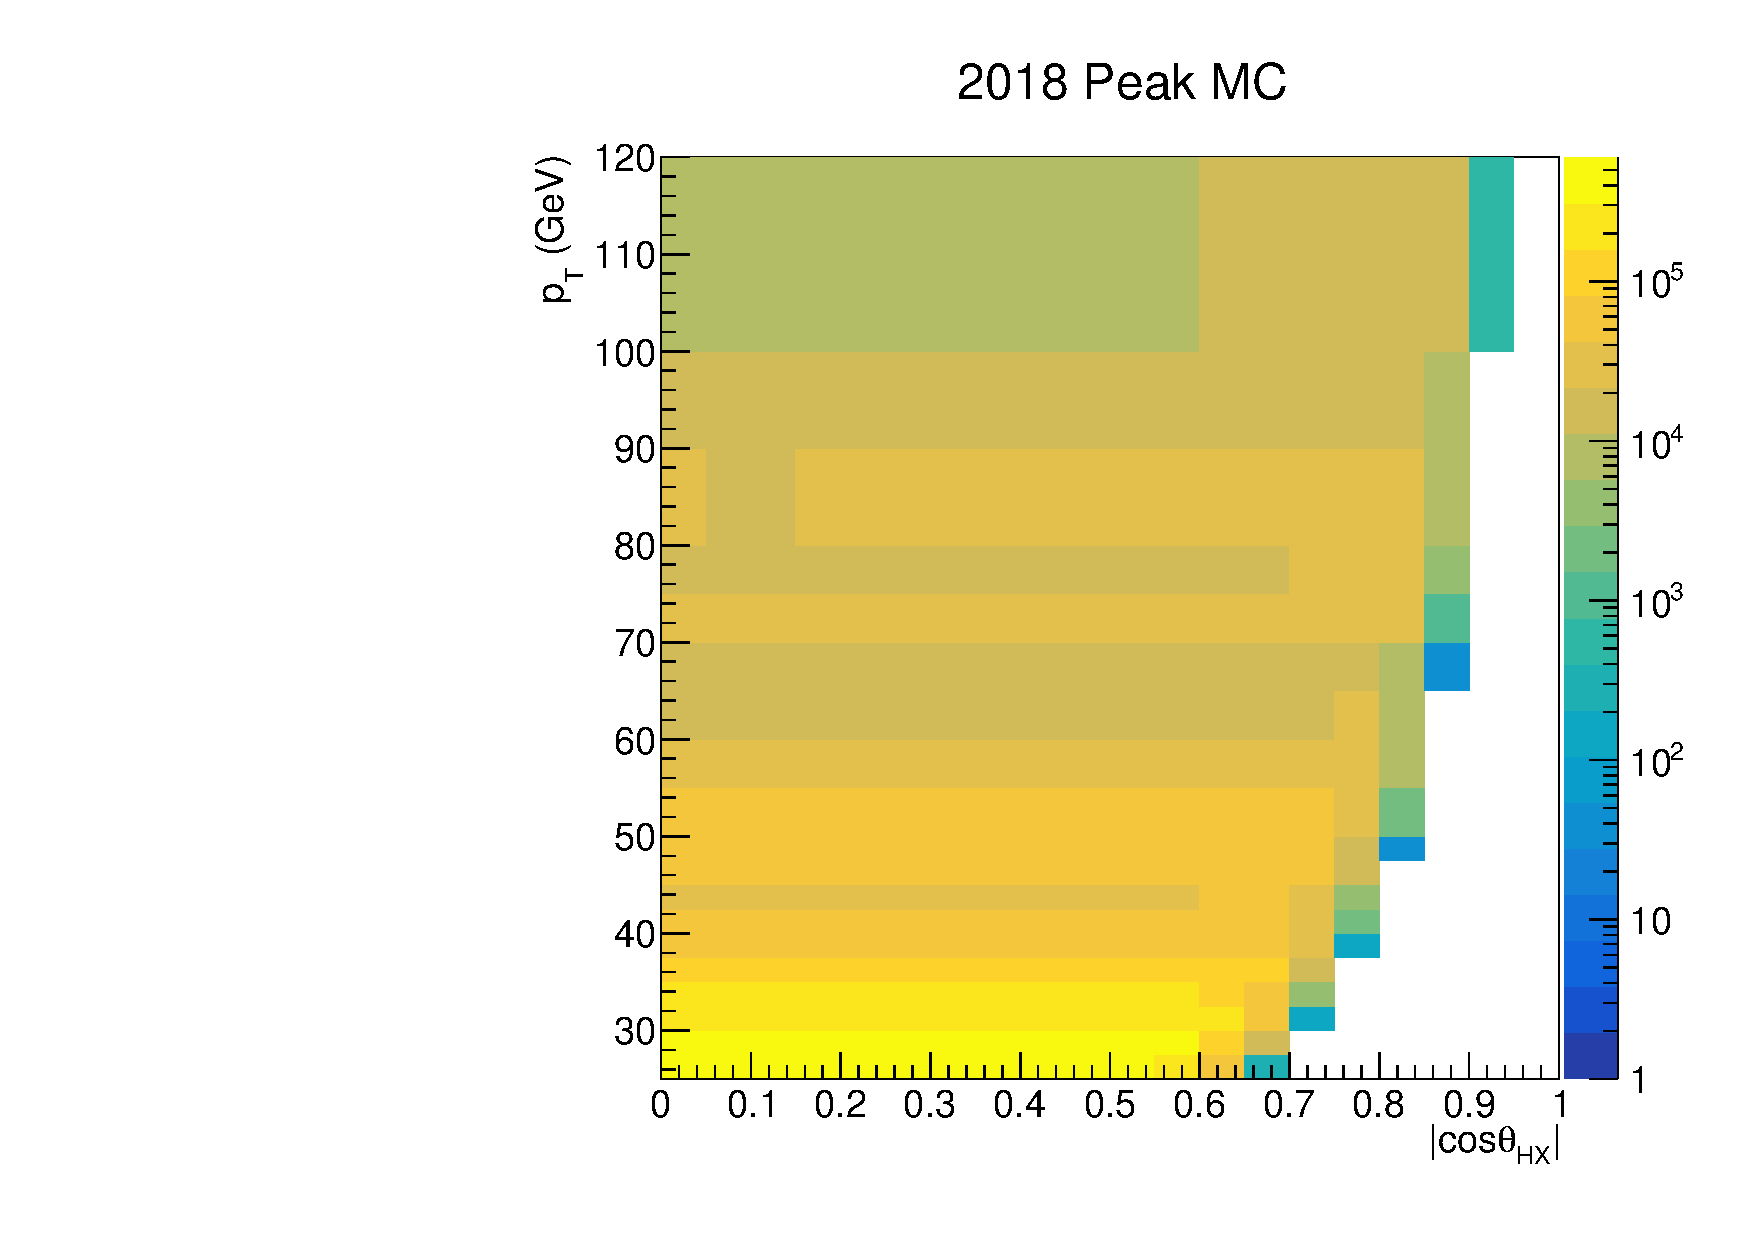
\includegraphics[width=0.48\textwidth]{Figures/chapter3/mc_2d_plot.pdf}
\caption{Two-dimensional \jpsi $(\abscosth,\pt)$ distributions for 2018 
Peak data (left) and signal-only MC (right).}
\label{fig:2Dmaps_data_vs_MC}
\end{figure}

Besides the expected (exponential) decrease in event yields as \pt increases,
which simply reflects the decreasing \pt-differential production cross section, 
the first observation that we can make from these figures is that the coverage in 
\abscosth extends to larger values when the dimuons have a larger \pt.
In fact, the requirement that \emph{both} muons must have $\pt > 5.6$\GeV 
implies that we cannot see in our sample any events where the two muons are
``back-to-back" in the helicity frame, 
blinding us from seeing the \costh regions close to $-1$ or $+1$.
As the dimuon \pt increases, the impact of the muon \pt cut becomes less important,
so that we see the measured \abscosth distribution extending towards higher
values of \abscosth, as shown in Fig.~\ref{fig:costCov}.
In other words, the maximum value of the \abscosth variable that we can probe
in our data increases with dimuon \pt, 
which is another good reason to perform the analysis as a function of \pt.

\begin{figure}[t]
\centering
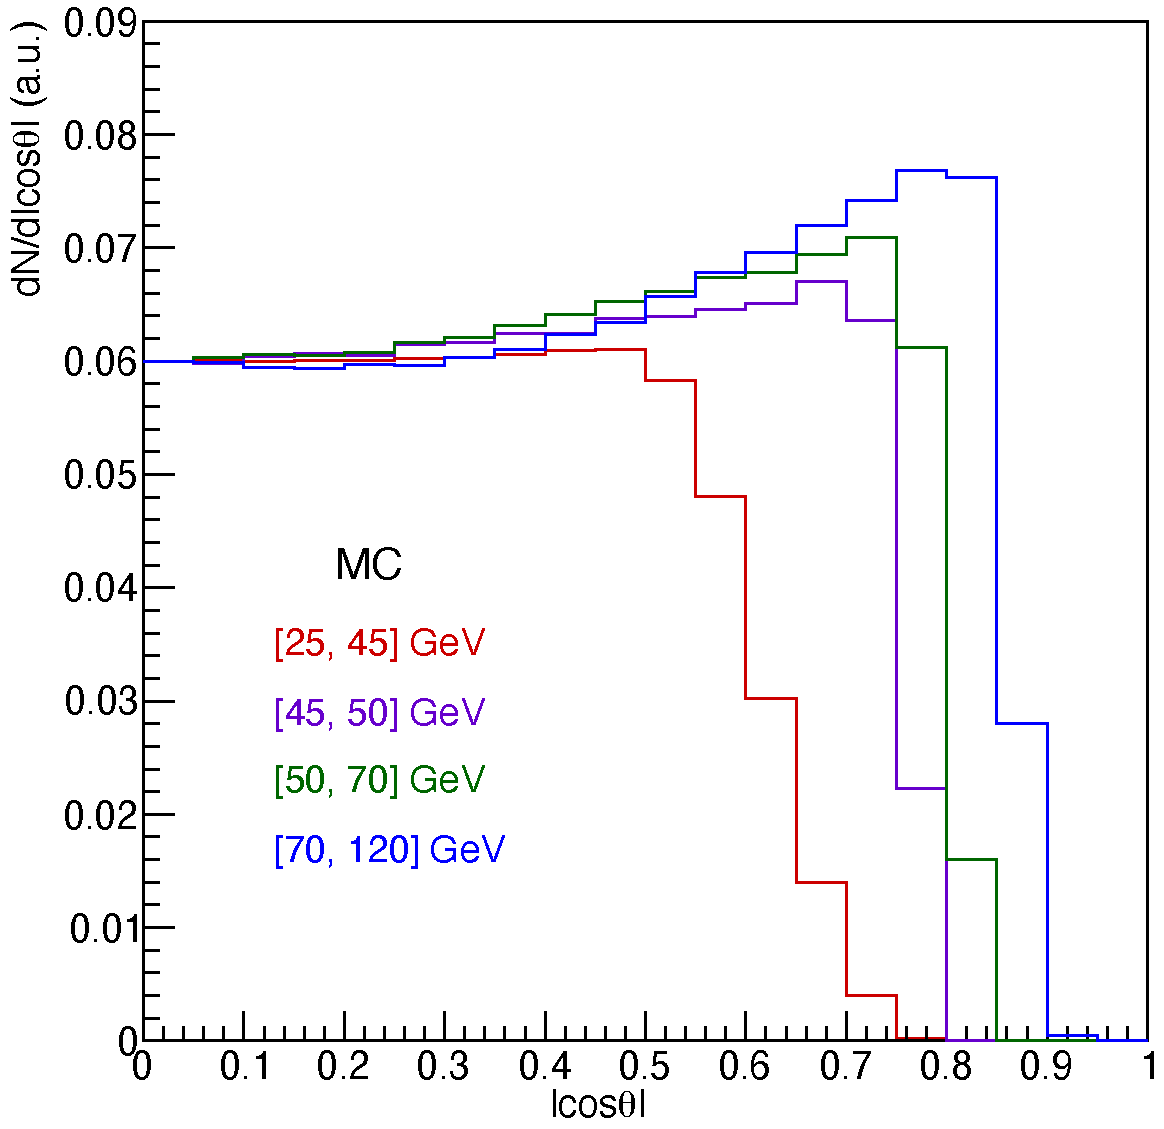
\includegraphics[width=0.45\textwidth]{Figures/chapter3/cos_MC2.pdf}
\caption{Simulated \abscosth distributions, in four \jpsi \pt ranges, 
showing that the \abscosth coverage increases with \pt.}
\label{fig:costCov}
\end{figure}

It is worth noting that this means that the polarization measurement becomes 
easier to perform as the \jpsi \pt increases (as long as we do not ``run out of events").
Indeed, the measurement of \lth benefits very significantly from the shape 
of the \costh distribution \emph{away from zero}.
Data that only cover a \costh range very close to zero are unable to
provide a faithful measurement of \lth.

Before acceptance-corrections, all the measured \costh distributions 
(in the HX frame) decrease towards the edges, $\abscosth \to 1$.
If we would fit them immediately with Eq.~\ref{eq:wfit}, we would probably get
negative \lth values, especially at low dimuon \pt, even if the \jpsi mesons
would be produced unpolarized or with transverse polarization.
As mentioned before, the analysis must be made using the data over MC ratios.
Figure~\ref{fig:2DmapsRatios} shows an example of such a ratio, 
for the Peak region, using the 2018 data and MC \jpsi samples.
The detection effects cancel in the ratio, so that 
its study will provide a reliable measurement of the polarizations.
Indeed, the polarization is the only effect that is present in the
measured distributions and not in the simulated ones, so that it
is the only possible cause of the (potential) non-flatness of the ratios.

\begin{figure}[h]
\centering
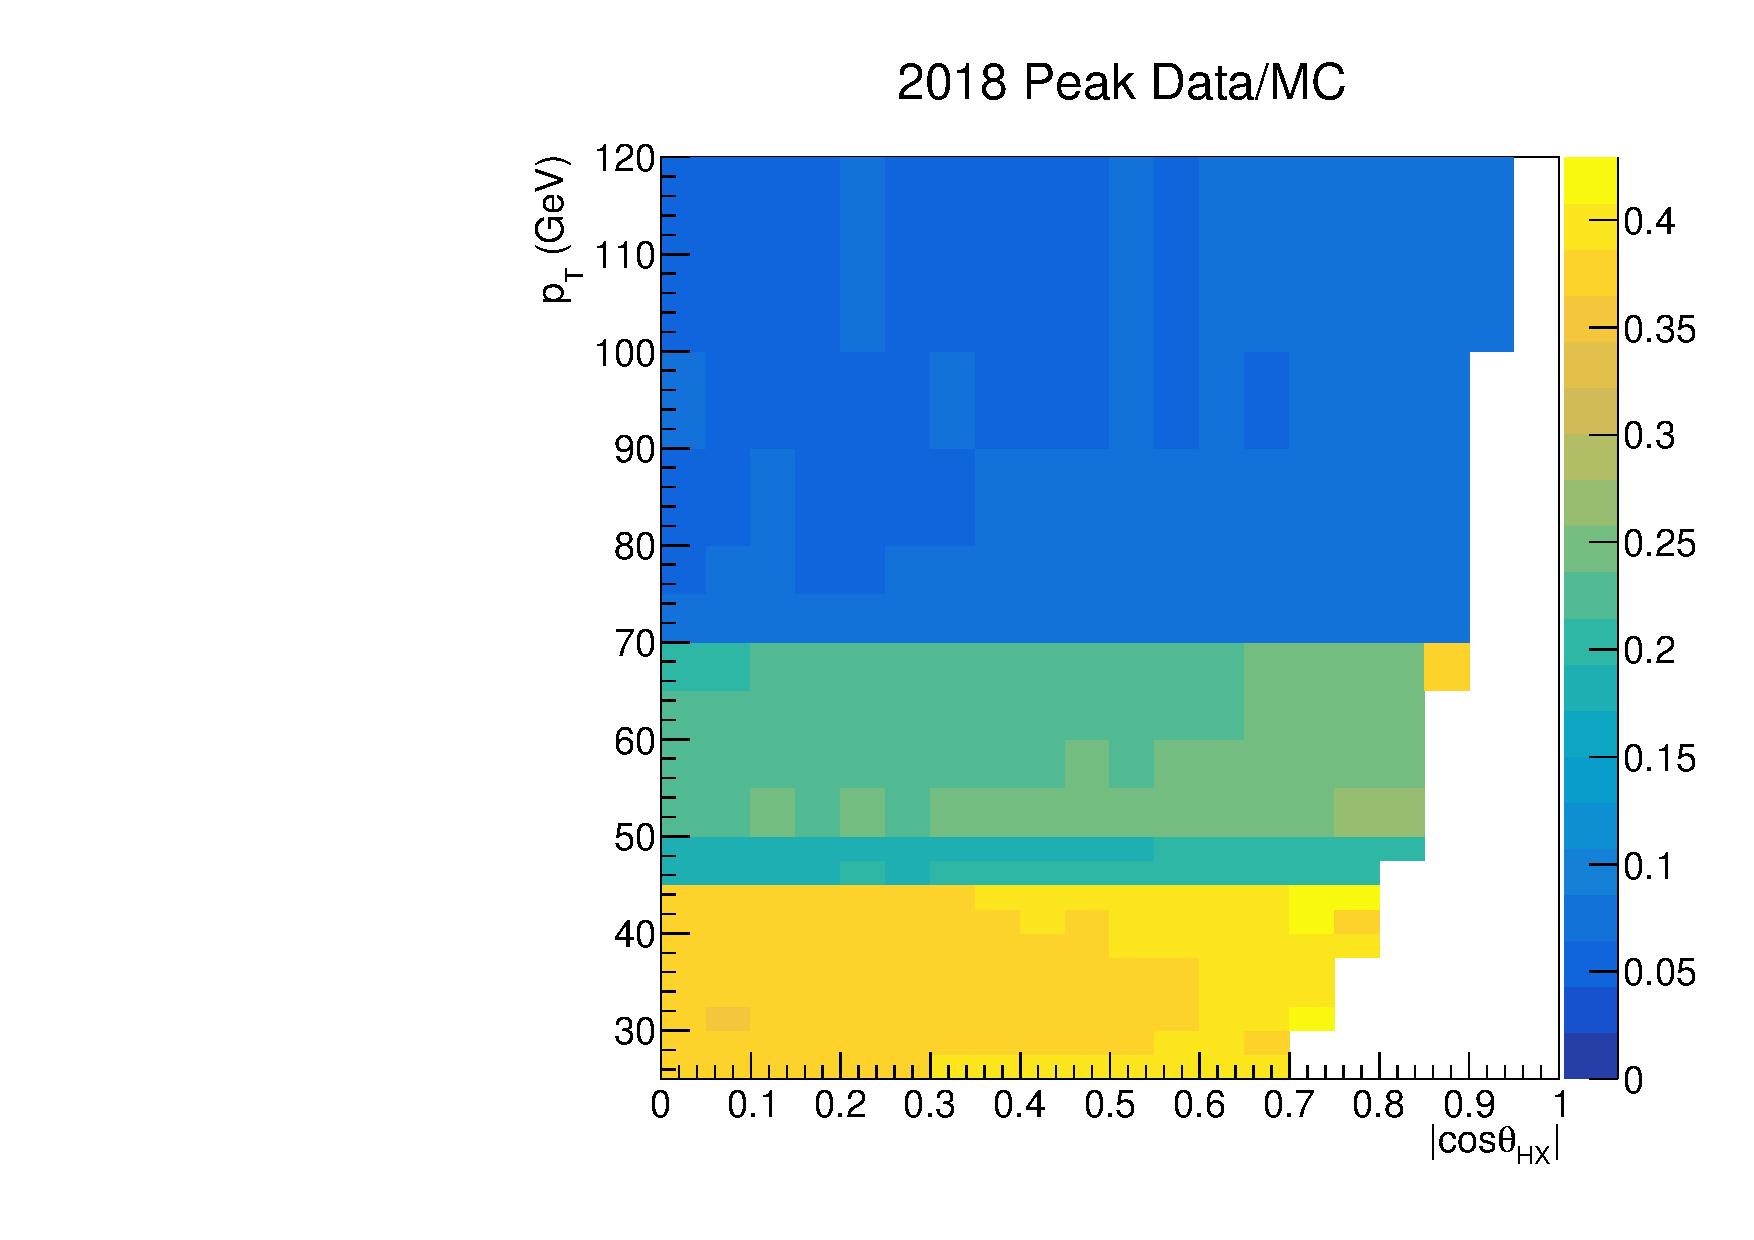
\includegraphics[width=0.48\textwidth]{Figures/chapter3/ratio_Peak.pdf}
\caption{Data over MC ratio of the \jpsi $(\abscosth,\pt)$ 2D distributions
for the Peak region, using the 2018 samples.}
\label{fig:2DmapsRatios}
\end{figure}

\vfill\newpage

Figure~\ref{fig:2Dmaps_psip} shows the equivalent, for the \psip events,
of the panels shown in Figs.~\ref{fig:2Dmaps_data_vs_MC} 
and~\ref{fig:2DmapsRatios}.

\begin{figure}[t]
\centering
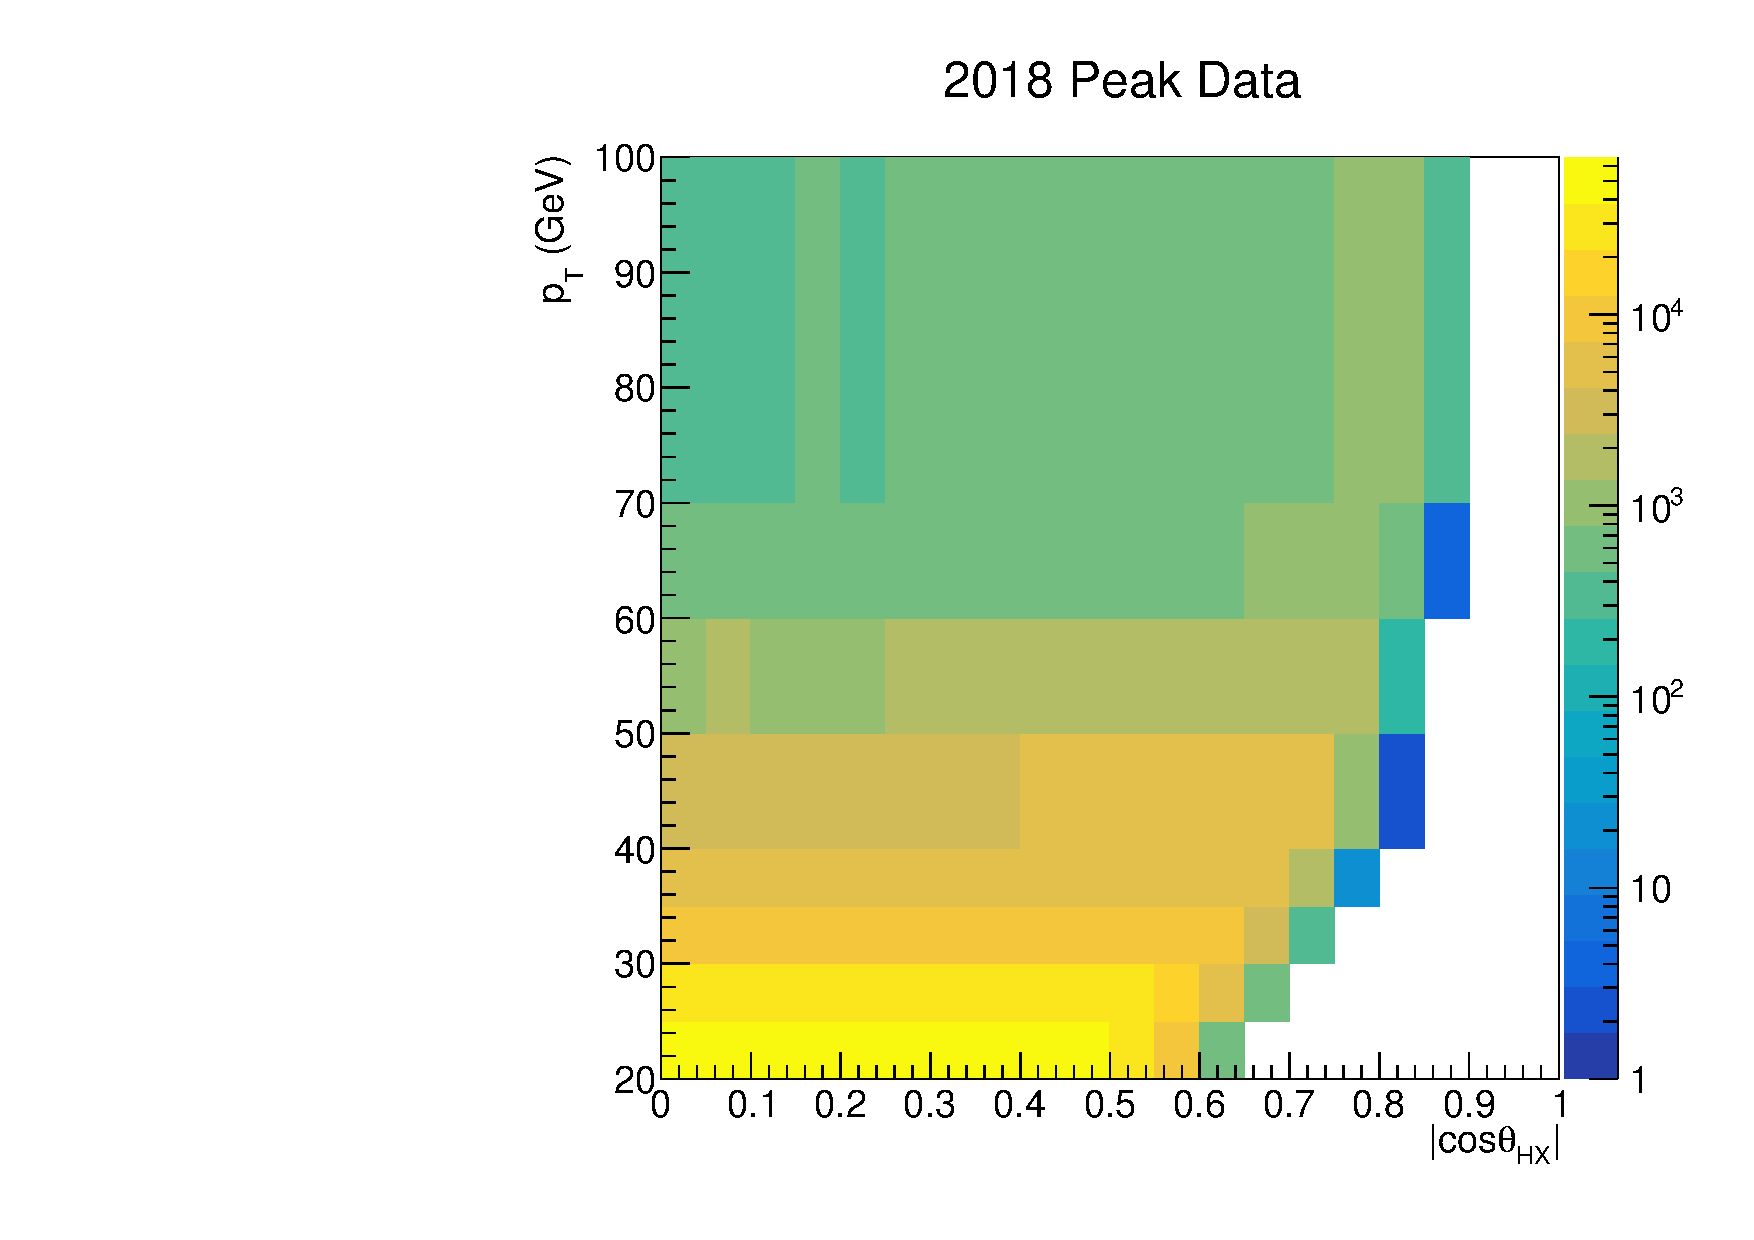
\includegraphics[width=0.48\textwidth]{Figures/chapter3/data_2d_plot_psip.pdf}
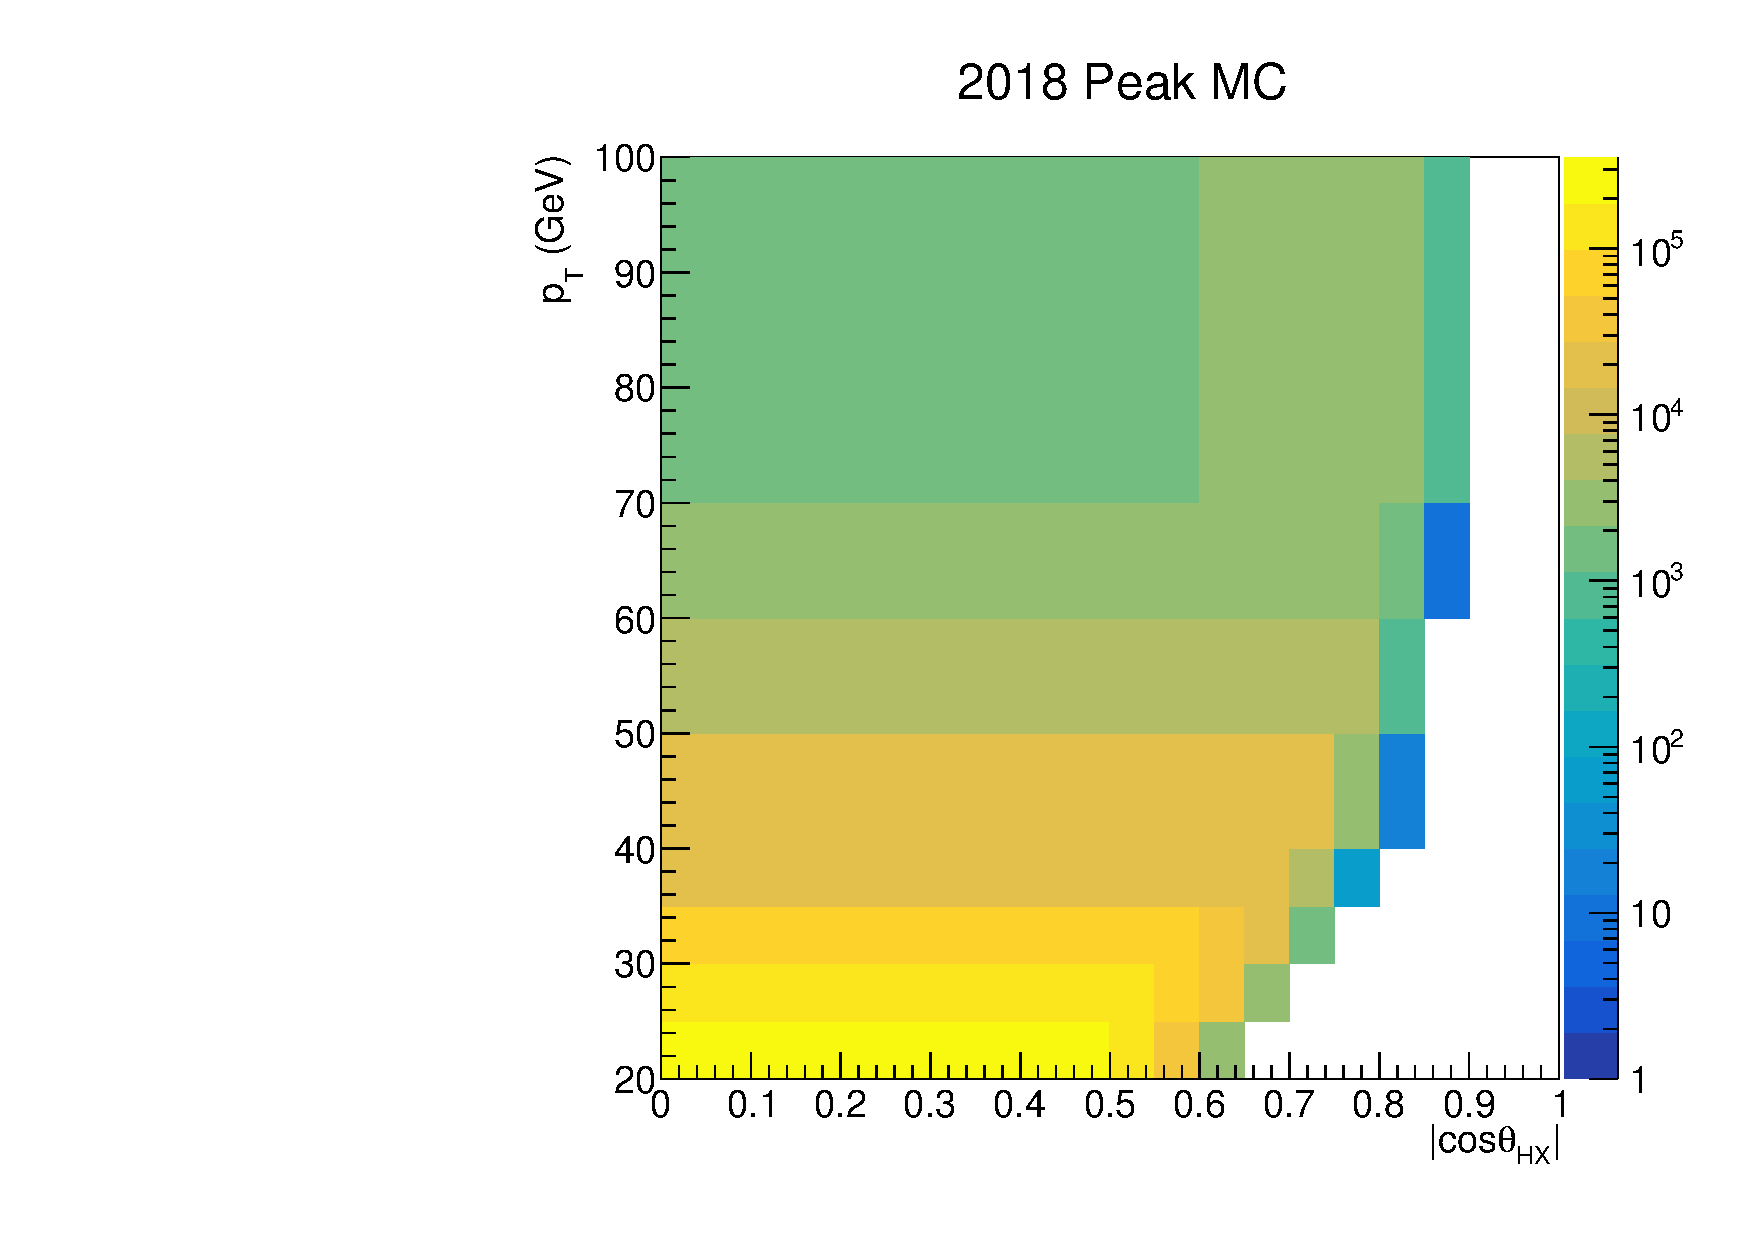
\includegraphics[width=0.48\textwidth]{Figures/chapter3/mc_2d_plot_psip.pdf}
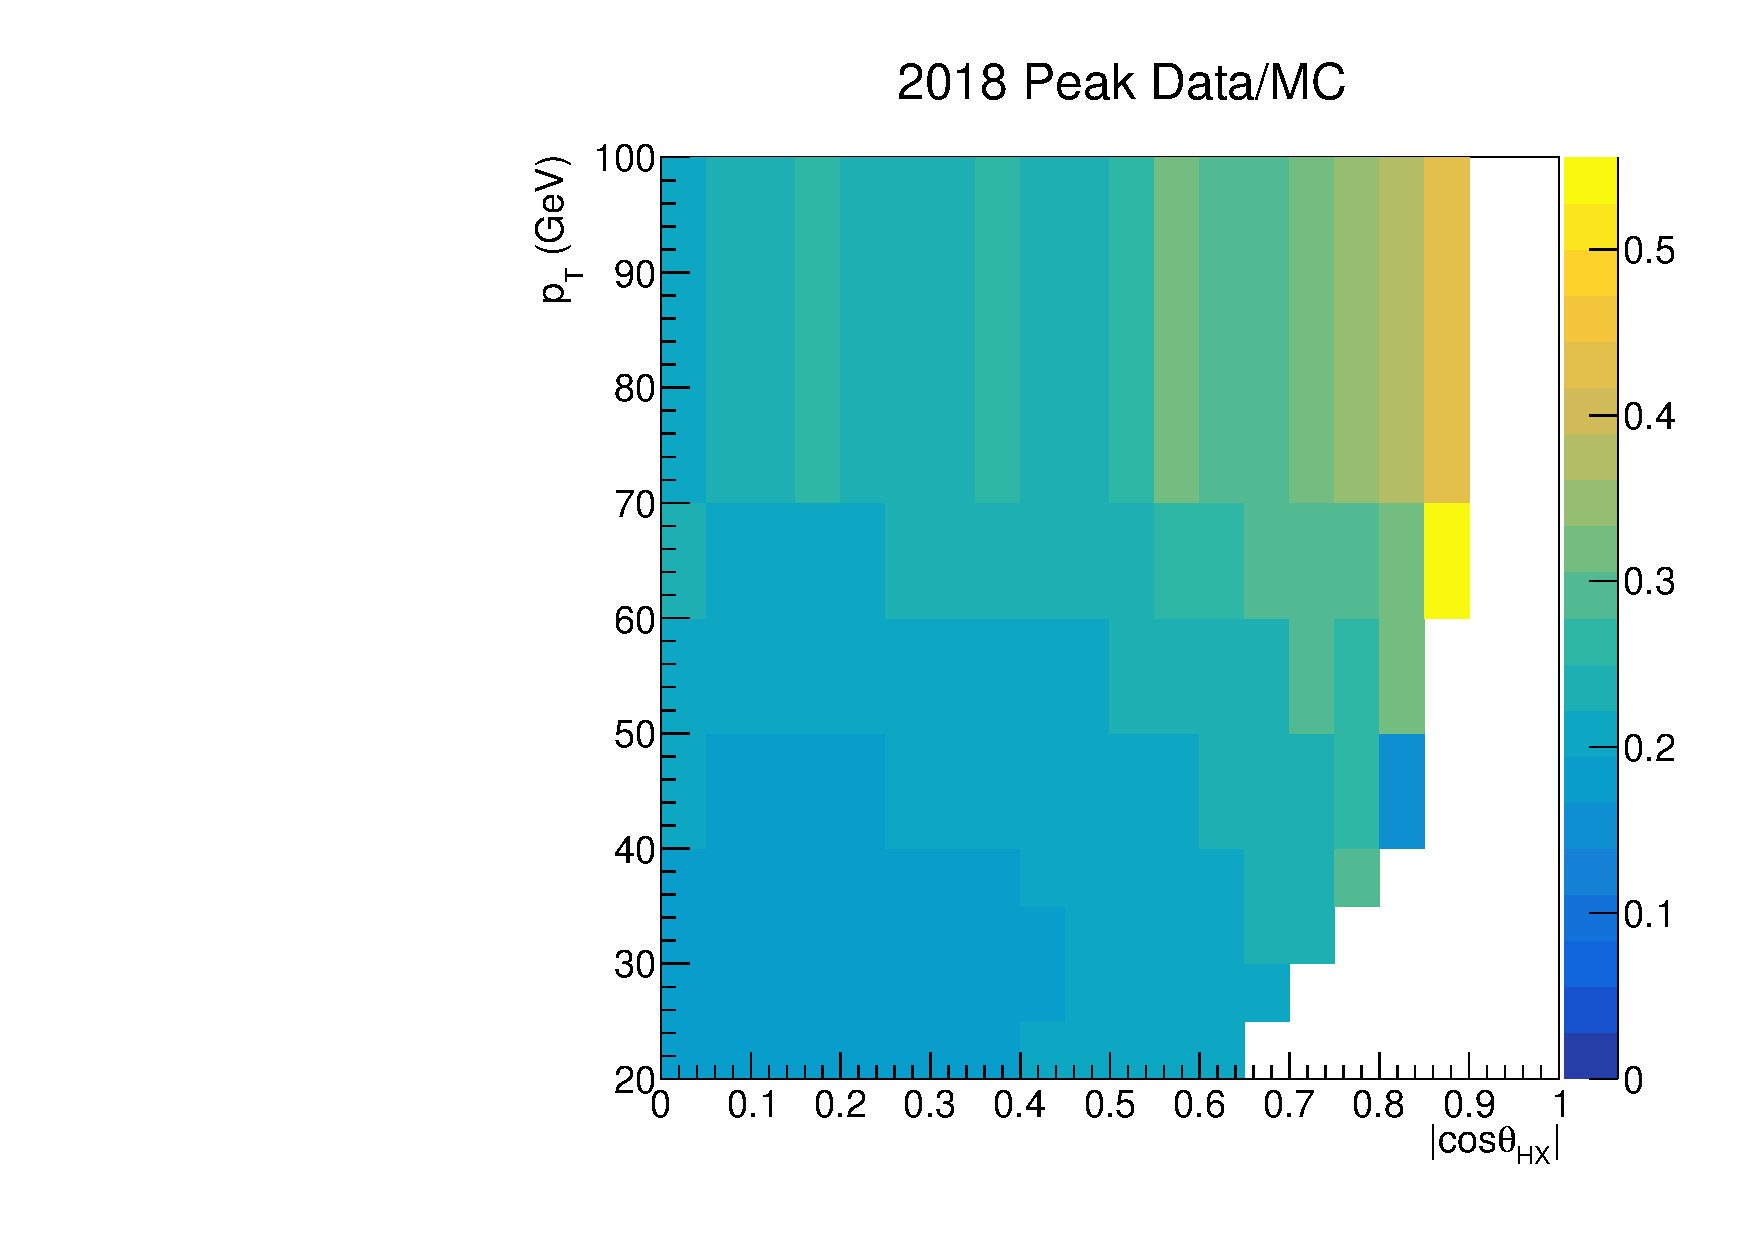
\includegraphics[width=0.48\textwidth]{Figures/chapter3/ratio_Peak_psip.pdf}
\caption{Two-dimensional \psip $(\abscosth,\pt)$ distributions for 2018 
Peak data (top left), signal-only MC (top right), and data over MC ratio (bottom).}
\label{fig:2Dmaps_psip}
\end{figure}

\vfill\newpage

To ensure stable and reliable fit results, the $1 + \lth \cos^2\theta$ function 
is fitted within a \abscosth range that excludes the most extreme values, 
where the distribution (corrected for acceptance and efficiency effects) 
is the ratio of two steeply falling distributions and, hence,
might be affected by spurious ``edge effects".

Before we go into more complex descriptions of the analysis procedures, 
it is worth noting that, even without doing any fits, 
a direct look at the measured \jpsi \abscosth distributions,
shown in Fig.~\ref{fig:costh_full} for the Peak, NP and MC cases, integrated over \pt,
is sufficient to see that the Peak dimuons are transversely polarized 
while the NP dimuons, instead, are longitudinally polarized.
This observation can be easily made by comparing the Peak and NP shapes 
with that of the \emph{unpolarized MC} distribution, taken as reference.

\begin{figure}[h]
\centering
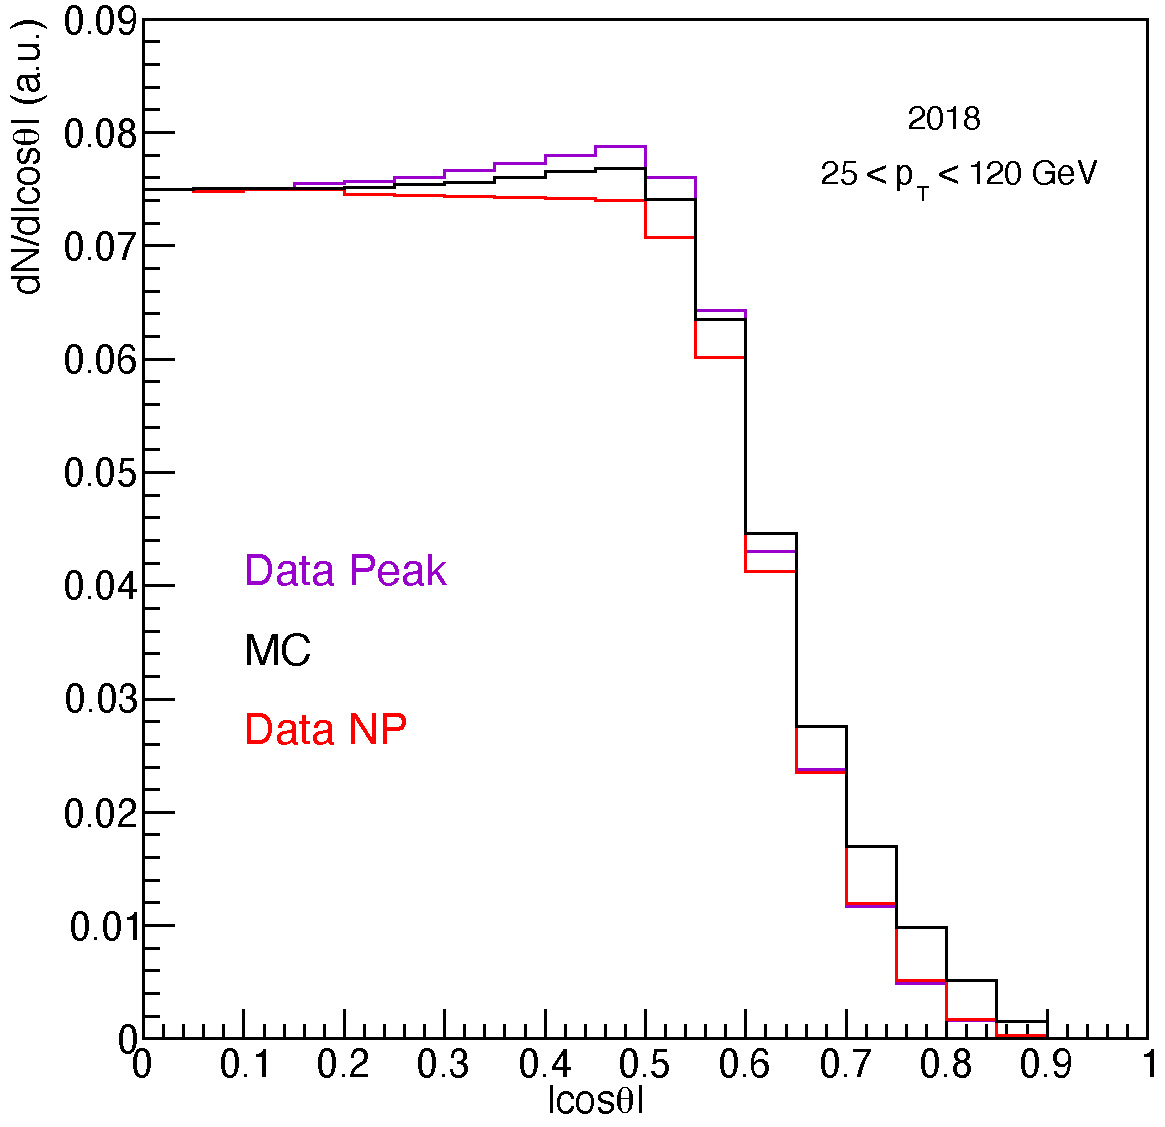
\includegraphics[width=0.48\textwidth]{Figures/chapter3/cos_full2.pdf}
\caption{Measured Peak (purple) and NP (red) \jpsi \abscosth distributions
compared to the MC simulated (unpolarized) distribution (black),
immediately illustrating the transverse or longitudinal polarizations of the
measured samples.}
\label{fig:costh_full}
\end{figure}

\vfill\newpage

Also for pedagogical purposes, 
we will now illustrate the polarization measurement for the dimuons in the 
Peak and NP regions, without subtracting any of the background terms.
While these are not to be seen as final physics results, 
they have the advantage of showing, in a simple way,
how the procedure translates the angular distributions in the \lth polarization parameter.

Figure~\ref{fig:Peak-NP-pol}-left shows the \abscosth distribution of the 2018 Peak (violet) 
and NP (red) dimuons, for the 42.5--45\GeV dimuon \pt bin, 
an intermediate \pt bin, suitable for this illustration.
As mentioned before, 
these distributions reflect not only the polarization of the respective dimuons 
but also the detector acceptance effects.
The right-side panel of the same figure shows the ratio between the measured 
distributions and the simulated one, for the same data taking period and \pt bin.
In these ratios, the detector effects cancel out and we can proceed to the fit step,
using the function $1 + \lth \cos^2 \vartheta$.
The results are $\lth = 0.157 \pm 0.016$ for the Peak dimuons and 
$\lth = -0.178 \pm 0.015$ for the NP dimuons, for this specific \pt bin, 
of the 2018 data.

\begin{figure}[h]
\centering
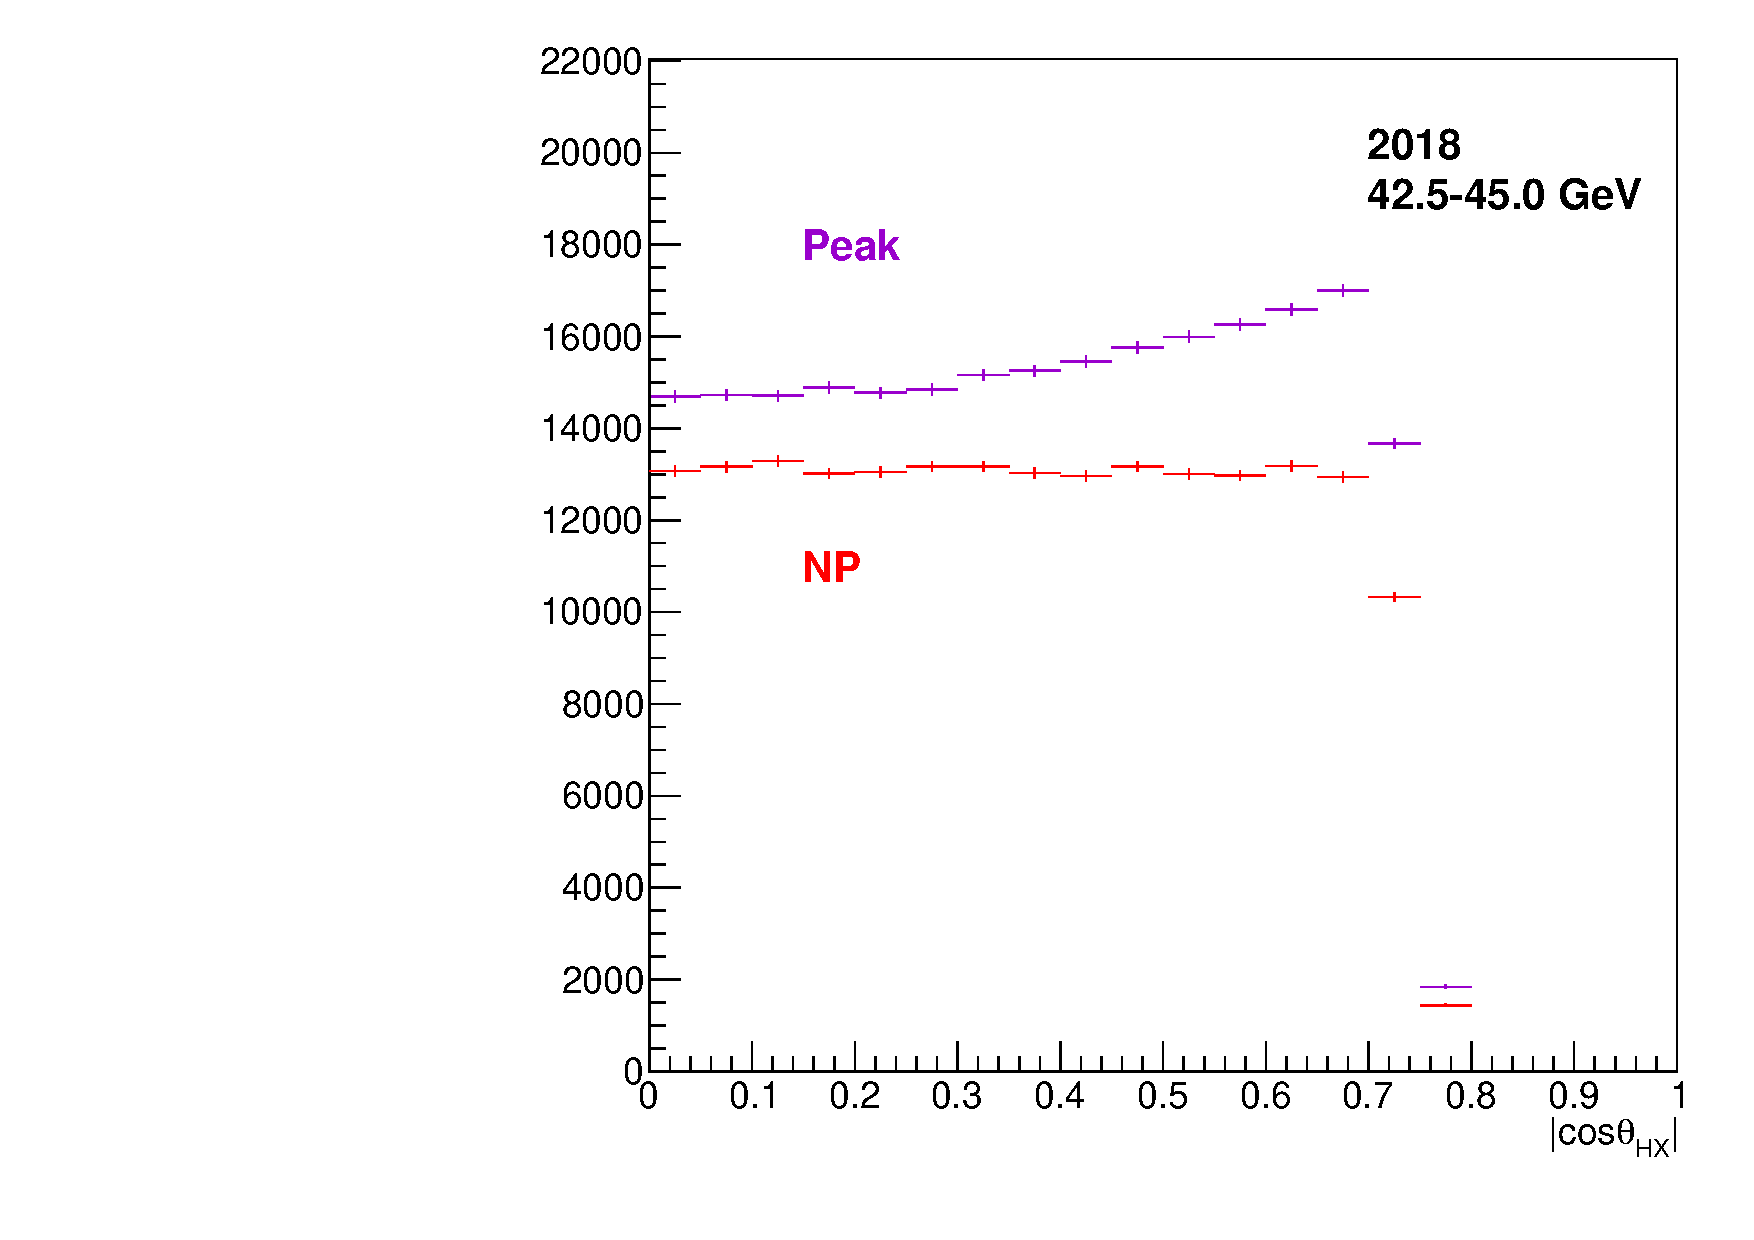
\includegraphics[width=0.48\textwidth]{Figures/chapter3/bin2B_7.pdf}
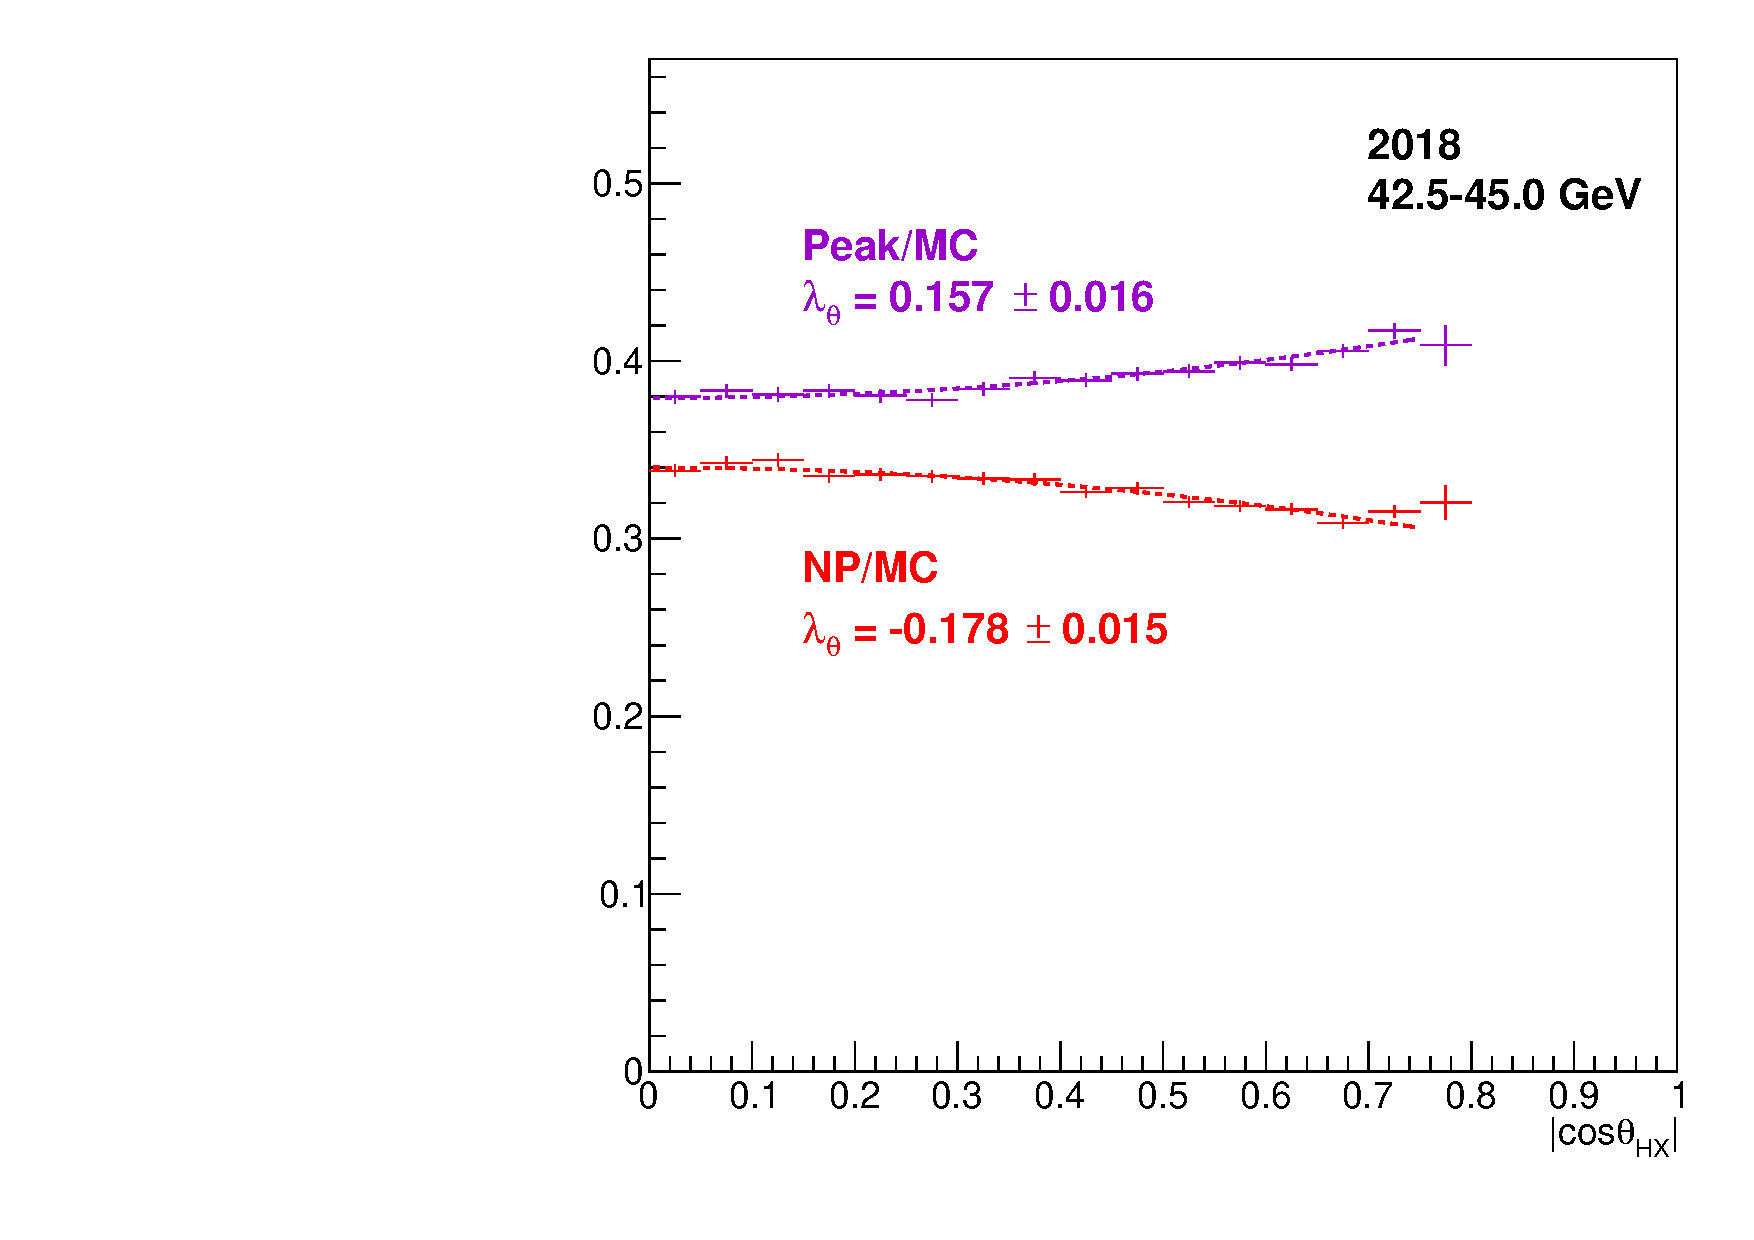
\includegraphics[width=0.48\textwidth]{Figures/chapter3/bin2F_7.pdf}
\caption{Illustration of the analysis procedure: 
the Peak and NP \abscosth distributions (left) 
and the Peak/MC and NP/MC ratios (right), 
in the 42.5--45\GeV \pt bin of the 2018 data.}
\label{fig:Peak-NP-pol}
\end{figure}

\vfill\newpage

\begin{figure}[t]
\centering
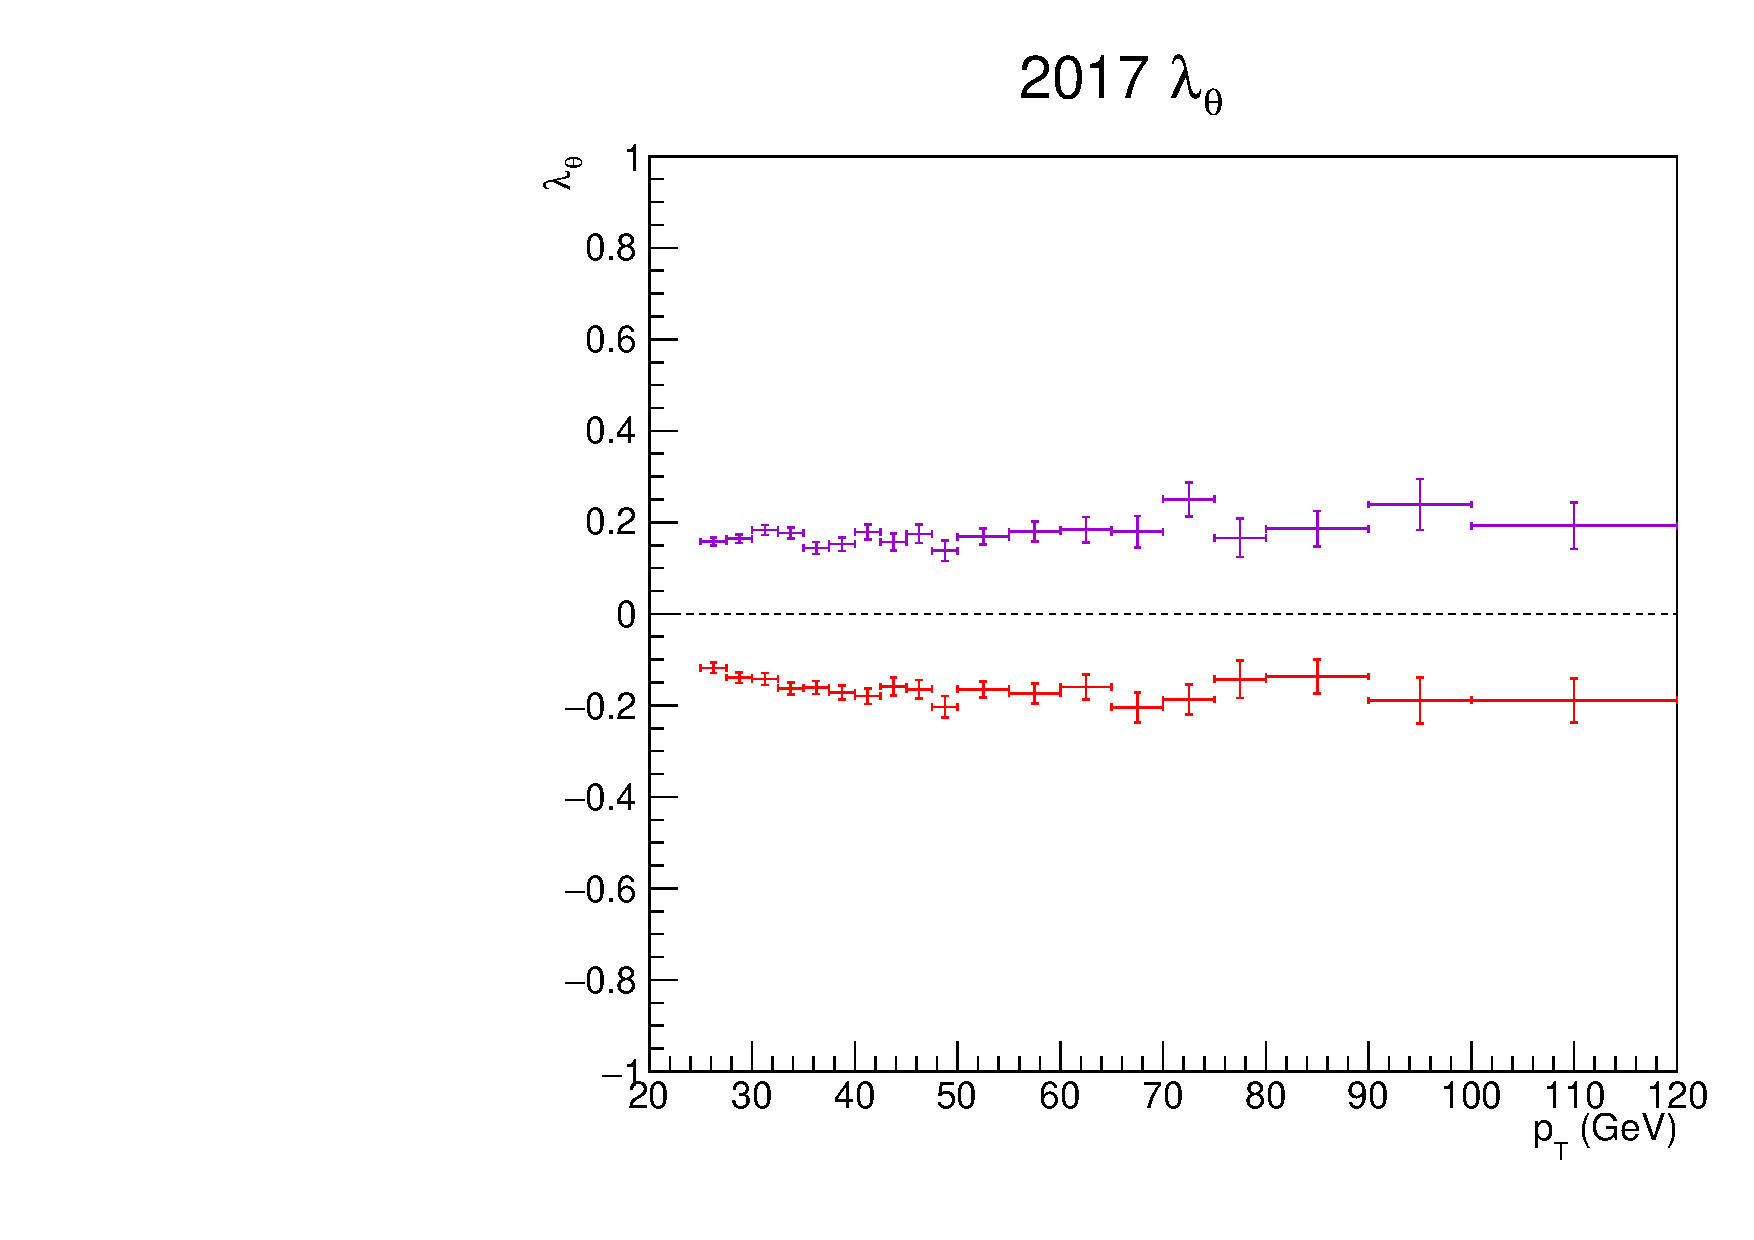
\includegraphics[width=0.48\textwidth]{Figures/chapter3/lth2_17.pdf}
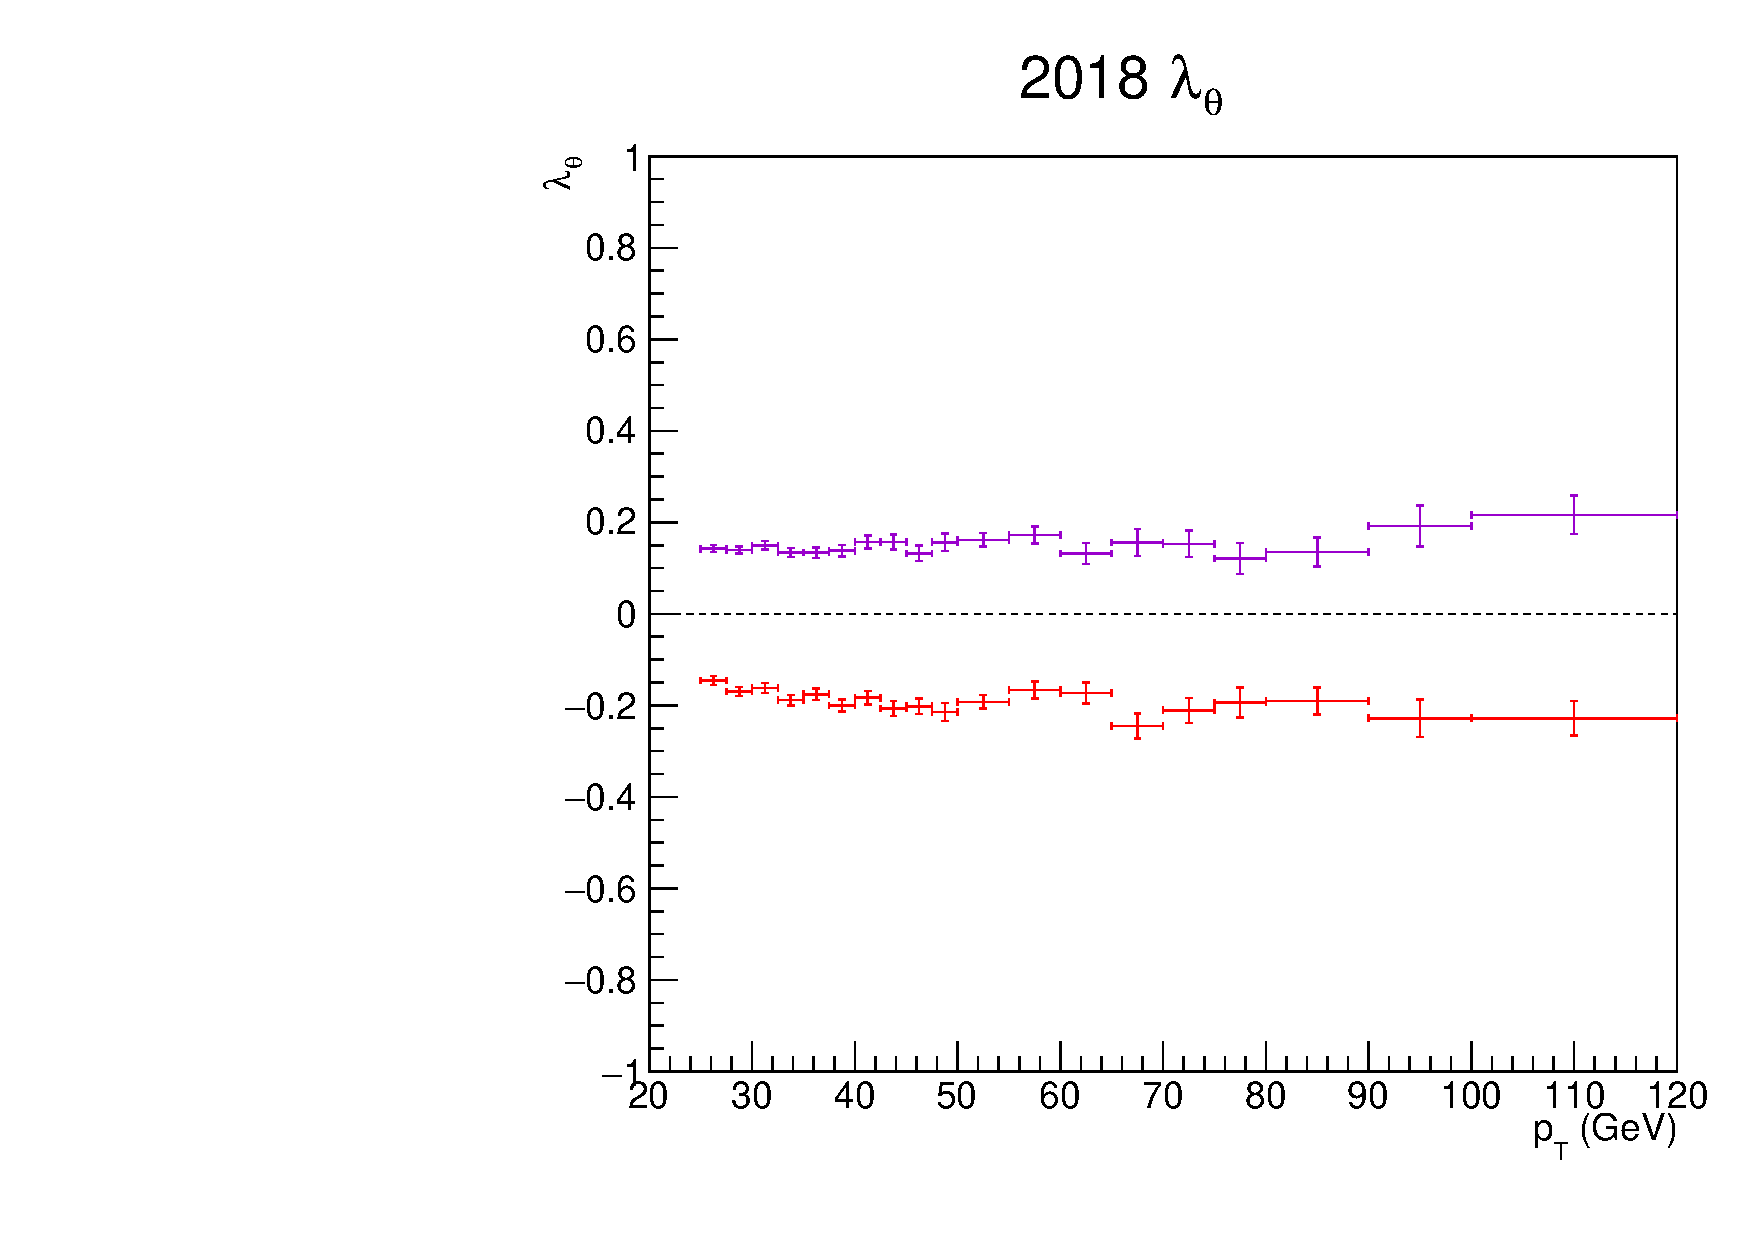
\includegraphics[width=0.48\textwidth]{Figures/chapter3/lth2_18.pdf}
\caption{Illustration of the analysis procedure: 
the \lth values measured for the Peak (violet) and NP (red) dimuons 
collected in 2017 (left) and 2018 (right), 
before subtracting the background contributions.}
\label{fig:Peak-NP-lth}
\end{figure}

Applying this procedure to all the \pt bins and to both periods of data taking 
provides the values of \lth as a function of \pt shown in Fig.~\ref{fig:Peak-NP-lth}.

As previously mentioned, 
these results are only shown in here because we believe that it is informative
to see how the polarization values, vs.\ \pt, 
are obtained from the measured angular distributions,
before we proceed into the background subtraction steps.

In particular, the NP \lth values shown in Fig.~\ref{fig:Peak-NP-lth} 
cannot be seen as measurements of the polarizations of the non-prompt \jpsi mesons, 
resulting from B decays, because the NP event sample is contaminated by
non-prompt ``mass-continuum" muon pairs 
that happen to have an invariant mass between 3.0 and 3.2\GeV
but are not produced by \jpsi decays.
This background contribution needs to be evaluated, 
using the NP~LSB and NP~RSB sideband regions mentioned above, 
and then subtracted, before we achieve the final physics result.

Analogously, the \lth values obtained from the Peak region cannot be interpreted 
as a measurement of the prompt \jpsi polarization, because it is affected by the 
(prompt) mass-continuum muon pairs and also by the \jpsi mesons produced by B mesons
that decay with a very small lifetime value, so that they are counted in the PR region
($|c\tau| < 50\,\mu$m).

Nevertheless, while not yet being physical measurements, 
these \lth versus \pt trends offer a useful first approximation of the final results,
under the (reasonable) assumption that 
the backgrounds are relatively small and/or have a negligible 
impact on the polarization measurement.

In particular, it is interesting to note that the measured values 
extend over a very broad \pt range 
and have uncertainties that are much smaller than those we have seen 
in the analysis of the 7\TeV data (Fig.~\ref{fig:BPH13003}).

\vfill\newpage

The next step is to measure the \lth polarization parameter of the \emph{signal} 
prompt and non-prompt \jpsi and \psip mesons. 
For simplicity, we will describe the procedures for the \jpsi case;
the \psip measurement is done in the same way.
For the prompt case, and as just mentioned, 
we must subtract from the Peak sample two sources of background:
the underlying mass continuum background caused by (uncorrelated) muon pairs, 
evaluated by integrating, inside the \jpsi peak region, 
the continuum distribution defined by the left and right sidebands;
and the \jpsi mesons resulting from decays of B mesons,
evaluated by integrating, inside the PR region, 
the lifetime distribution of the NP term, defined by the NP region.
This background subtraction must be done, naturally, as a function of \pt.
The procedure is represented by the following equation:
\begin{equation}
\begin{split} 
\text{Peak}(\abscosth,\pt) 
&= (1 - f_{\rm NP}(\pt) - f_{\rm Bg}(\pt)) \cdot \psi_\mathrm{PR}(\abscosth,\pt) \\
&+ f_{\rm NP}(\pt) \cdot \text{NP}(\abscosth,\pt) \\
&+ f_{\rm Bg}(\pt) \cdot \text{Bg}(\abscosth,\pt) \, .
\end{split}
\label{eq:bkgSub_psi_PR}
\end{equation}

Or, equivalently, by:
\begin{equation}
\begin{split} 
\psi_\mathrm{PR}(\abscosth,\pt) 
&= \frac{1}{1 - f_{\rm NP}(\pt) - f_{\rm Bg}(\pt)} \times \\
& [ \text{Peak}(\abscosth,\pt) 
- f_{\rm NP}(\pt) \cdot \text{NP}(\abscosth,\pt) 
- f_{\rm Bg}(\pt) \cdot \text{Bg}(\abscosth,\pt) ] \, .
\end{split}
\label{eq:bkgSub2}
\end{equation}

In order to determine the physically-relevant $\psi_\mathrm{PR}(\abscosth,\pt)$ term from the 
immediately measurable $\text{Peak}(\abscosth,\pt)$ term,
we need to evaluate the $\text{NP}(\abscosth,\pt)$ and $\text{Bg}(\abscosth,\pt)$ distributions,
as well as the fractions of events in the Peak region which are due to these two sources,
$f_{\rm NP}(\pt)$ and $f_{\rm Bg}(\pt)$.
We do that through the analysis of the dimuon mass and lifetime distributions,
presented in the next chapter.

The procedure for the measurement of the signal non-prompt \jpsi polarization is
analogous but simpler 
because there is only one background term, the (non-prompt) continuum muon pairs:

\begin{equation}
\begin{split}
\text{NP}(\abscosth,\pt)
&= (1 - f_{\rm NPBg}(\pt)) \cdot \psi_{\rm NP}(\abscosth,\pt) \\
&+ f_{\rm NPBg}(\pt) \cdot \text{NPBg}(\abscosth,\pt) \, .
\end{split}
\label{eq:bkgSub_psi_NP}
\end{equation}


\vfill\newpage

The $\text{Peak}(\abscosth,\pt)$ and $\text{NP}(\abscosth,\pt)$ distributions 
are directly obtained from the measured event samples.
The $\text{Bg}(\abscosth,\pt)$ and $\text{NPBg}(\abscosth,\pt)$
distributions are evaluated as a weighted average of the (PR or NP) LSB and RSB samples.
The fractions of background contributions, $f_{\rm Bg}$ and $f_{\rm NP}$, 
are determined by fitting the dimuon mass and lifetime distributions, respectively.
Figure~\ref{fig:mass-and-lt-illustration} provides a graphical illustration of these
two backgrounds.

\begin{figure}[h]
\centering
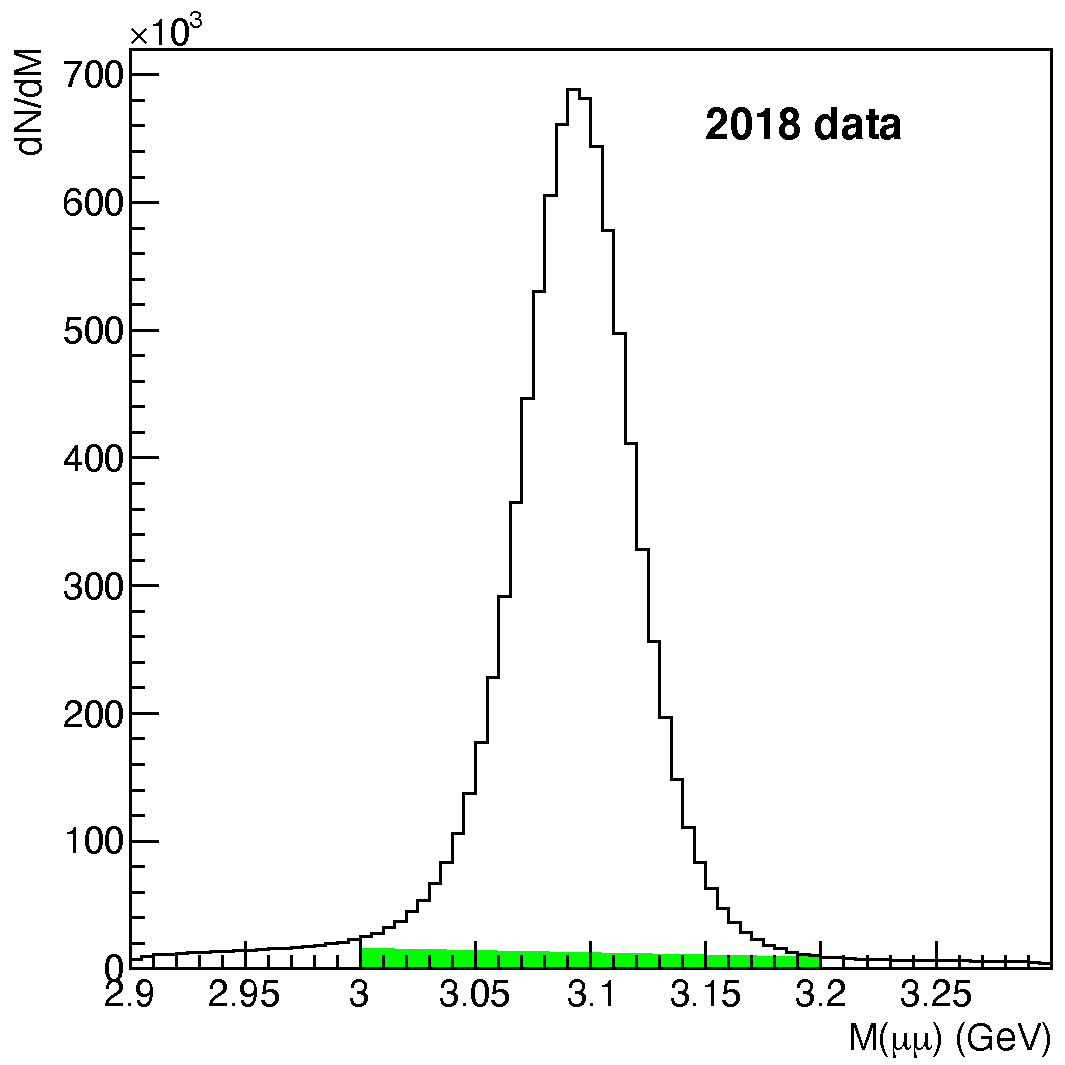
\includegraphics[width=0.48\textwidth]{Figures/chapter3/mass_continuum_background.pdf}
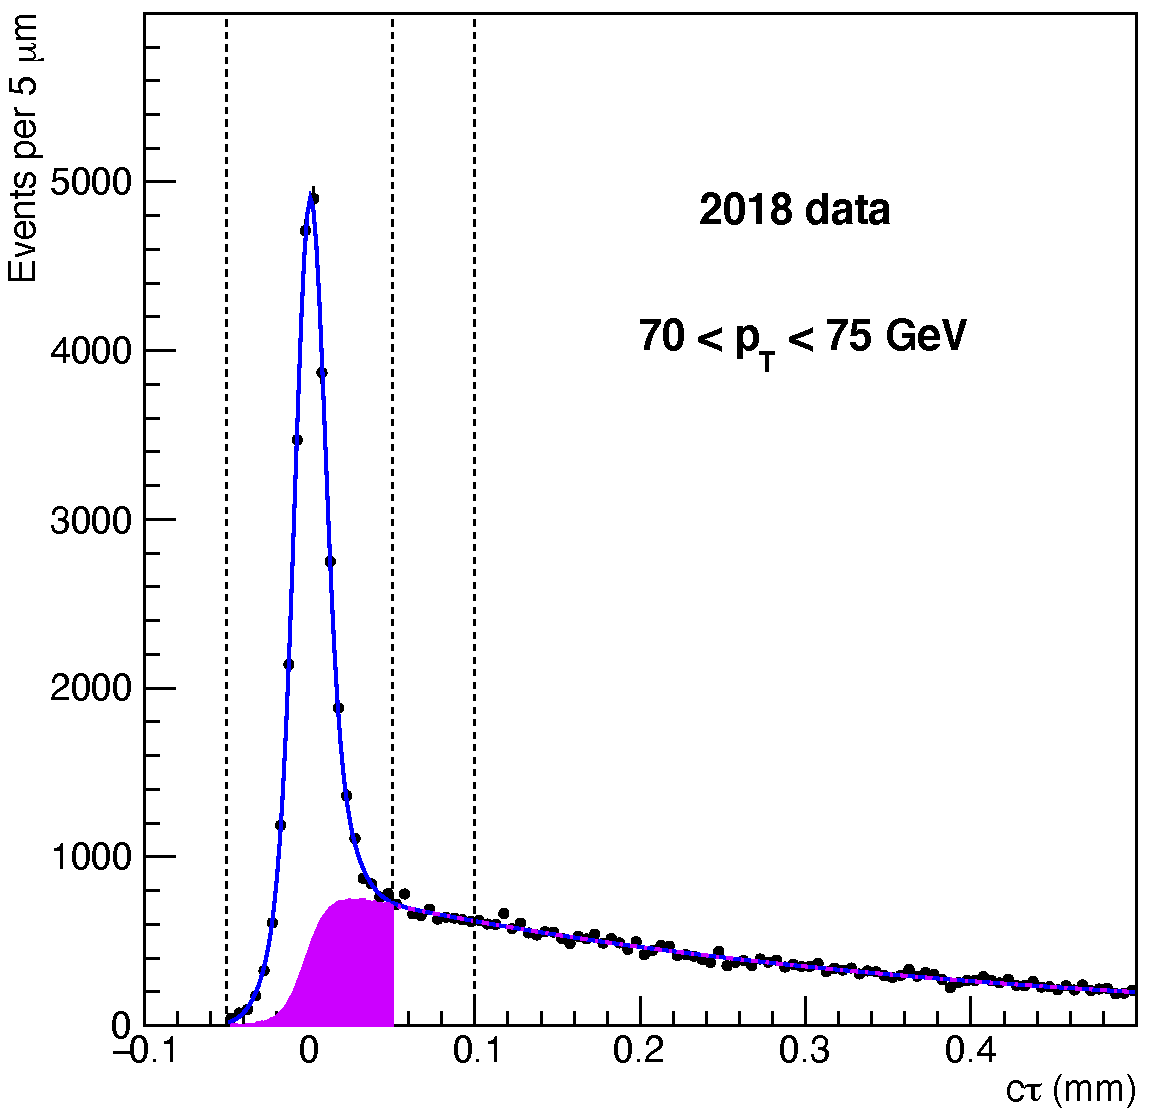
\includegraphics[width=0.48\textwidth]{Figures/chapter3/ltfit2.pdf}
\caption{Examples of measured dimuon mass and lifetime distributions,
using the 2018 \jpsi sample, meant to illustrate the shape and magnitude of the
mass and lifetime backgrounds under the prompt \jpsi peak.}
\label{fig:mass-and-lt-illustration}
\end{figure}

\vfill\newpage

Before we move on to the study of the dimuon mass and lifetime distributions, 
we should clarify that we have done several comparisons between the 2017 and 2018 samples, 
including independent fits of the dimuon mass and lifetime distributions of each of those samples,
and arrived at the conclusion that the two samples lead to distributions that are 
in perfect agreement with each other, within uncertainties.
This observation means that we can perform 
the dimuon mass and lifetime fits using the combined ``Run 2" event sample.
In this way, some free parameters can be fitted with less statistical fluctuations
and we can see more precisely if they depend or not on the dimuon \pt, for example.

Residual variations between the two event samples, if any, 
are covered by assigning systematic uncertainties evaluated from the 
differences between the results independently obtained for each year.
This applies, independently, to the prompt and non-prompt \jpsi and \psip measurements.

Adding both years, the event yields, per 2D region and \pt range, 
are collected in the Tables~\ref{tab:yields-jpsi-Run2} and~\ref{tab:yields-psip-Run2}, 
for the \jpsi and \psip cases, respectively.

\begin{table}[h]
\centering 
\caption{Event yields of the measured and simulated \jpsi samples,
adding the 2017 and 2018 sets, per \pt range (in GeV).}
\label{tab:yields-jpsi-Run2}
\small
\begin{tabular}{cl|cccc|c}
\hline
\multicolumn{2}{c}{2017} & $[25, 45]$ & $[45, 50]$ & $[50, 70]$ & $[70, 120]$ & $[25, 120]$ \\
\hline
\multirow{6}{*}{\rotatebox[origin=c]{90}{Data}} 
& Prompt signal region (Peak) & 13.362 M & 0.517 M & 0.698 M & 0.180 M & 14.757 M \\
& Non-prompt region (NP) & 9.629 M & 0.445 M & 0.626 M & 0.168 M & 10.869 M \\
& Prompt left mass SB (PRLSB) & 113.8 k & 5.2 k & 7.7 k & 2.4 k & 129.2 k \\
& Prompt right mass SB (PRRSB) & 132.4 k & 7.3 k & 11.3 k & 4.0 k & 155.0 k \\
& Non-prompt left mass SB (NPLSB) & 159.1 k & 7.4 k & 10.2 k & 2.8 k & 179.5 k \\
& Non-prompt right mass SB (NPRSB) & 168.1 k & 8.0 k & 11.0 k & 3.0 k & 190.0 k \\
\hline
MC & only Peak region & 41.492 M & 3.145 M & 3.759 M & 2.874 M & 51.270 M \\
\hline
\end{tabular}
\end{table}

\begin{table}[ht]
\centering 
\caption{Event yields of the measured and simulated \psip samples,
adding the 2017 and 2018 sets, in the full \pt range.}
\label{tab:yields-psip-Run2}
\small
\begin{tabular}{cl|c}
\hline
\multicolumn{2}{c}{2017} & $[20, 100]$ \\
\hline
\multirow{6}{*}{\rotatebox[origin=c]{90}{Data}} 
& Prompt signal region (Peak) & 2.130 M \\
& Non-prompt region (NP) & 1.351 M \\
& Prompt left mass SB (PRLSB) & 404.8 k \\
& Prompt right mass SB (PRRSB) & 459.5 k\\
& on-prompt left mass SB (NPLSB) & 367.6 k\\
& Non-prompt right mass SB (NPRSB) & 141.6 k \\
\hline
MC & only Peak region & 10.349 M  \\
\hline
\end{tabular}
\end{table}
